Requirements Management and Engineering (RE\&M) is taught, both in industry and academia. The availability of open source SE-tools, and Eclipse-based tools in particular, created some interest for using those tools for teaching. 

%===============================================================================
\section{Vision}
%===============================================================================

The vision of this project is to create:\marginpar{(mj) Contributors, feel free to comment via margin comments!}

\begin{enumerate}
\item A set of teaching materials that is actively used; 
\item Which is embedded in a larger SE context; and
\item Which explicitly focuses on applying RE. 
\end{enumerate}

%===============================================================================
\section{Scope}
%===============================================================================

The scope is the creation of teaching materials, centered around a case study, based on existing methods and tools. This is visualized in Figure~\ref{fig:scope}.

\begin{figure}[h!]
  \centering
  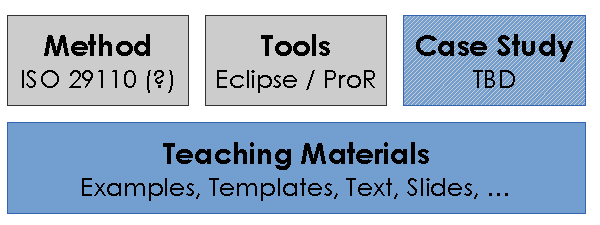
\includegraphics[width=\textwidth]{../se-images/teaching-overview.pdf}
  \caption{Scope of the SE teaching materials}
  \label{fig:scope}
\end{figure}

ISO 29110 looks promising as the foundation for the method. Eclipse-based tools in general, and ProR for requirements engineering in particular, will be used. We are currently looking for a suitable case study, ideally using something that already exists. The focus will be on the creation of shared teaching materials. 

%===============================================================================
\section{Tools}
%===============================================================================

A central idea of this project is the use of freely available tools, as we cannot expect students to invest in expensive tools.  Tools will be based on Eclipse.  Figure~\ref{fig:v-model} depicts a simplified V-Model, depicting the pictures we could employ.

\begin{figure}[h!]
  \centering
  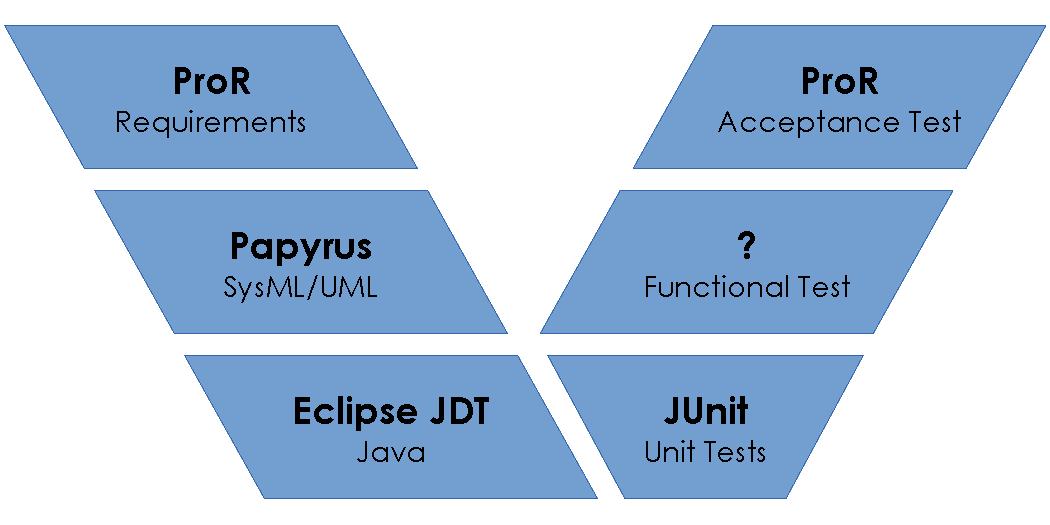
\includegraphics[width=\textwidth]{../se-images/v-model.pdf}
  \caption{Tools used in this course}
  \label{fig:v-model}
\end{figure}

\begin{info}
In a ``real'' project, there would be many more tools and artifacts.  We will keep tools and artifacts to a minimum, in order not to overwhelm the students.
\end{info}

%===============================================================================
\section{Background}
%===============================================================================

This project started in July 2014 as a discussion on \href{https://www.linkedin.com/groupItem?commentID=-1&item=5890782095432781827&type=member&gid=128312&view=}{LinkedIn}.  Thank you to all contributors!

%===============================================================================
\section{License}
%===============================================================================

No license has been selected yet! Please defer from using this content until a license has been selected.  It will probably be CC-BY --- the Creative Commons license that allows commercial reuse.


